% Generated from tex/chapters/ch04/07_実務上の考慮.tex for the SWEBOK structure tree
\subsubsection{統合}

統合とは、個別に作られた関数、クラス、部品、サブシステムを一つのシステムへ組み合わせることである。さらに、他のソフトウェアやハードウェアと接続することも統合に含まれる。

統合には、段階的統合と一括統合がある。一括統合は、すべての部品ができてからまとめて結合する方法であり、ビッグバン統合とも呼ばれる。問題発見が遅れやすい。段階的統合は、小さな単位から順に組み合わせる方法であり、エラーの場所を特定しやすく、進捗を把握しやすい。

段階的統合では、まだ存在しない部品の代役として、スタブ、ドライバ、モックオブジェクトなどの足場が必要になることがある。現代では、継続的統合によって、変更のたびに自動的にビルドとテストを行うことが広く使われる。

\begin{figure}[htbp]
\centering
\IfFileExists{assets/generated_figures/ch04/fig-ch04-07.png}{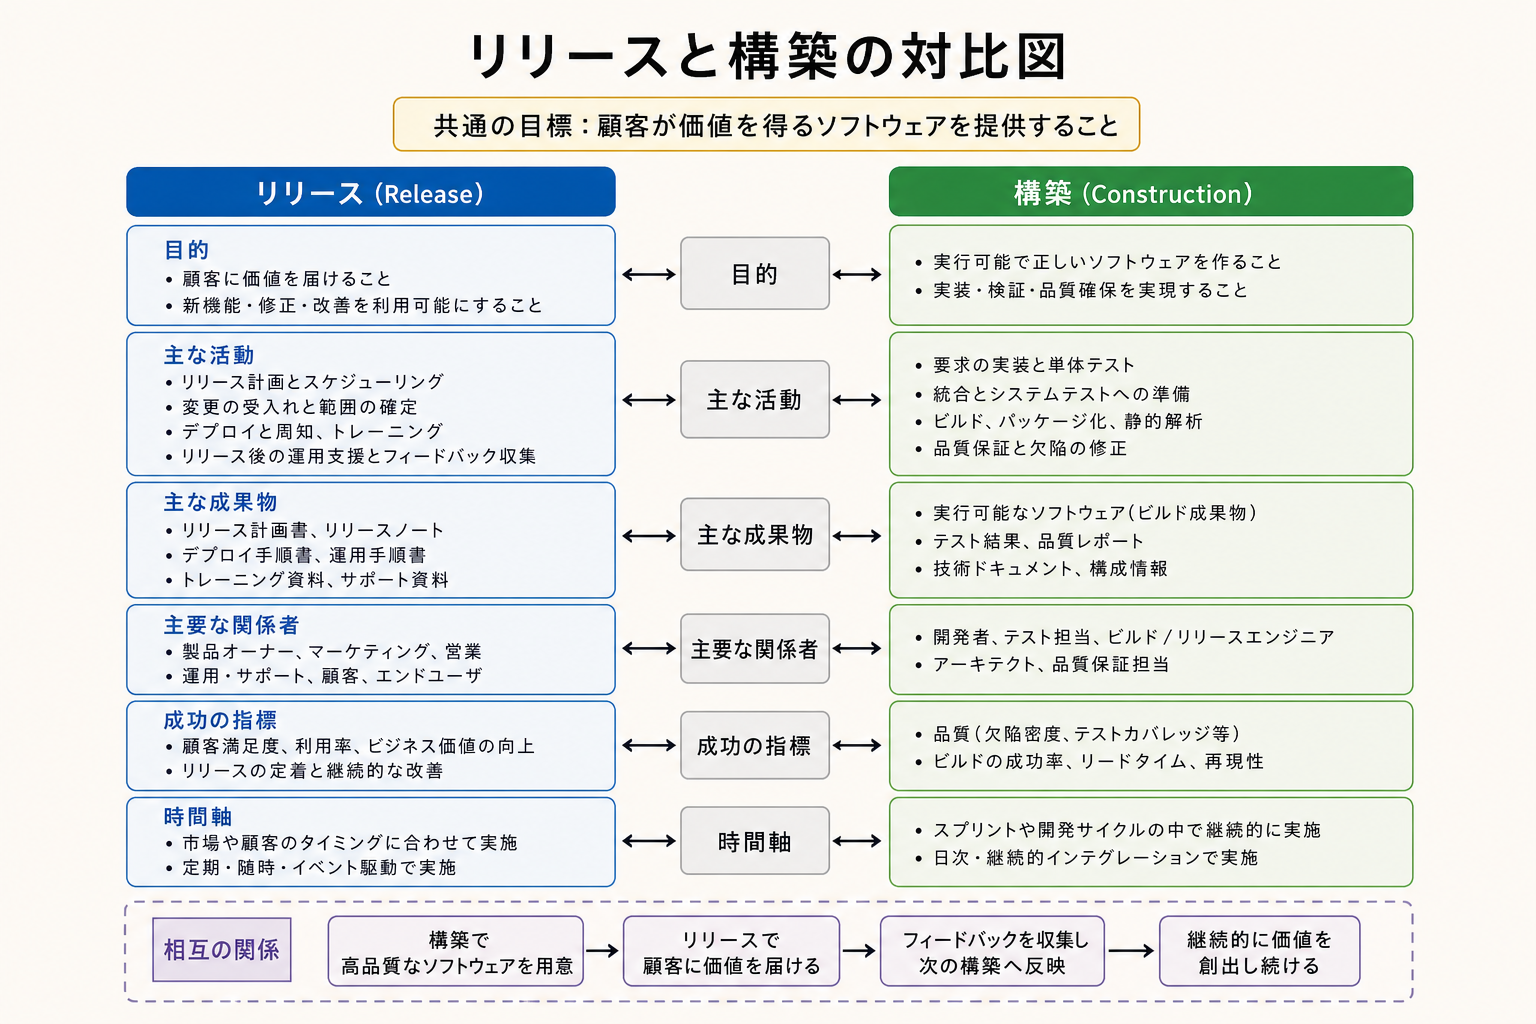
\includegraphics[width=0.96\linewidth]{assets/generated_figures/ch04/fig-ch04-07.png}}{\fbox{\parbox[c][48mm][c]{0.9\linewidth}{\centering 画像生成待ち\\段階的統合と継続的統合の流れ}}}
\caption{段階的統合と継続的統合の流れ}
\label{fig:ch04-07}
\end{figure}
